\documentclass[a4paper,12pt]{article}
\usepackage [utf8x]{inputenc}
\usepackage[czech]{babel}
\usepackage{graphicx}
\usepackage{amsmath}
\usepackage{siunitx}
\usepackage{xspace}
\usepackage{url}
\usepackage{indentfirst}
\usepackage[margin=22mm]{geometry}
\usepackage{esvect}
\usepackage{ragged2e}
\usepackage{tikz,pgf}
\usepackage{bm}
\usepackage{perpage}
\usepackage{capt-of}

\graphicspath{
	{img/}
	{plots/}
}

\newcommand{\e}{\text{e}}


\MakeSorted{figure}
\newtoks\jmenopraktika \newtoks\jmeno \newtoks\datum
\newtoks\obor \newtoks\skupina \newtoks\rocnik \newtoks\semestr
\newtoks\cisloulohy \newtoks\jmenoulohy
\newtoks\tlak \newtoks\teplota \newtoks\vlhkost
\jmenopraktika={Paschenův zákon, katodový spád potenciálu v doutnavém výboji}  % nahradte jmenem vaseho predmetu
\jmeno={Radek Horňák, Lukáš Vrána}            
\datum={15. 3. 2022}        % nahradte datem mereni ulohy                           
\rocnik={2.}                  
\semestr={IV.}                 
\cisloulohy={6}    % cislo ulohy           

\begin{document}
	\begin{center}
		{\Large Přírodovědecká fakulta Masarykovy univerzity} \\
		\bigskip
		{\Large \bfseries PRAKTIKUM Z~FYZIKY PLAZMATU} \\
		\bigskip
		{\Large \the\jmenopraktika}
	\end{center}
	\bigskip
	\noindent
	\setlength{\arrayrulewidth}{1pt}
	\begin{tabular*}{\textwidth}{@{\extracolsep{\fill}} l l}
		\large {\bfseries Zpracovali:}  \the\jmeno  \hspace{20mm} \large  
		{\bfseries Naměřeno:} \the\datum\\[2.5mm]
		\hline
	\end{tabular*}

\section{Teorie}
\subsection{Paschenův zákon}

Z Townsendovy teorie lavin víme, že působením elektrického pole na zředěný plyn dochází k urychlování přítomných elektronů. Takto urychlené elektrony mohou ionizovat neutrální částice a vytvořit takzvanou Townsedovu lavinu. Počet elektronů vzniklých v důsledku Townsendovy laviny závisí exponenciálně na dráze $d$  

\begin{equation}
	n = n_0\,\e^{\alpha d}
	\label{1}
\end{equation}

kde $n_0$ je počet elektronů v~počátečním bodě $d = 0$ a $\alpha$ je první Townsendův nebo také ionizační koeficient. Elektrické pole můžeme charakterizovat napětím $U$ přiloženým mezi dvě rovinné elektrody, dráha $d$ je vzdálenost mezi elektrodami. Elektronovou lavinu doprovází vznik iontů, jejichž počet lze vyjádřit jako

\begin{equation}
	 n_i = n_0\,[e^{\alpha d}-1]
	\label{2}
\end{equation}

Ionty jsou polem urychlovány ke katodě, dopadají na ni a vyvolávají sekundární emisi elektronů. Tu popisuje Townsendův třetí koeficient neboli koeficient sekundární emise $\gamma$. Konkrétně udává průměrný počet elektronů emitovaných jedním iontem při jeho dopadu na katodu. Pomocí $\gamma$ lze vyjádřit podmínku zapálení výboje jako

\begin{equation}
	\gamma\,(e^{\alpha d } - 1) = 1
	\label{3}
\end{equation} 

tedy že v lavině musí být jedním primárním elektronem vytvořeno tolik iontů, které dopadem na katodu způsobí emisi jednoho nového elektronu. Ionizační koeficient $\alpha$ závisí na intenzitě elektrického pole 

\begin{equation}
	\frac{\alpha}{p} = A\,\e^{-\frac{Bp}{E}} 
	\label{4}
\end{equation}

kde $A = 1/\lambda_1$ a $B = U/\lambda_1$ jsou konstanty závislé na druhu plynu, $\lambda_1$ je střední volná dráha elektronů při jednotkovém tlaku. Dále lze (\ref{4}) přepsat jako

\begin{equation}
	\frac{\alpha}{p} = A\,\e^{-\frac{Bpd}{U}} 
	\label{5}
\end{equation}
Logaritmováním a úpravou (\ref{5}) získáme

\begin{equation}
	U = \frac{B\,pd}{\ln A - \ln \frac{\alpha}{d}}
	\label{6}
\end{equation}
Dosazením $\alpha\,d$ z (\ref{6}) do (\ref{3}), logaritmováním a dalšími úpravami dojdeme k tvaru

\begin{equation}
	A\,pd\,e^{-\frac{Bpd}{U_z}} = \ln \left(\frac{1}{\gamma} + 1\right)
	\label{7}
\end{equation}
kde $U_z$ je zápalné napětí výboje. Pro daný plyn a materiál katody položme pravou stranu (\ref{7})

\begin{equation}
	\ln \left(\frac{1}{\gamma} + 1\right) = C
	\label{8}
\end{equation}
Úpravami dostáváme

\begin{equation}
	U_z = \frac{B\,pd}{C' + \ln(pd)}
	\label{9}
\end{equation}

kde $C' = \ln C - \ln A$. Závislost $U_z = f (pd))$ se nazývá Paschenův zákon. Má charakteristický tvar, včetně minima nazývaného Stoletowův bod.

%odsazení zkontroluj

\subsection{Katodový spád potenciálu v doutnavém výboji}
Doutnavý výboj je druh výboje, jehož typický vzhled můžeme vidět na schématu na obr. \ref{glowdischarge}. V rozmezí tlaku 13-130\,\si{\pascal} v něm můžeme pozorovat střídající se temné nebo svítící oblasti. Elektron pohybující se ve výboji od katody k anodě získá dostatečnou energii k excitaci neutrálů až v oblasti katodové vrstvy, ta je tedy prví svítící oblastí. Následuje temný katodový prostor, protože elektrony s vysokou energií ionizují neutrály, k vzniku fotonů zde nedochází. Nově vzniklé elektrony ionizací s malou energií vytvoří další svítivou oblast, kterou nazýváme záporné světlo. Energie elektronů dále klesá a následuje Faradayův temný prostor. Na jeho konci vzrůstá intenzita elektrického pole, energie elektronů opět roste a jsou schopné excitačních svítivých srážek, viz kladný sloupec. Jak se blížíme k anodě, na konci kladného sloupce vzniká anodový spád potenciálu v důsledku prostorového náboje, elektrony vystupují z kladného sloupce s malou rychlostí. Jakmile překonají anodový temný prostor, mají opět dostatek energie na excitaci i ionizaci neutrálů a tak u anody pozorujeme anodové světlo.

\begin{figure}[h]
	\centering
	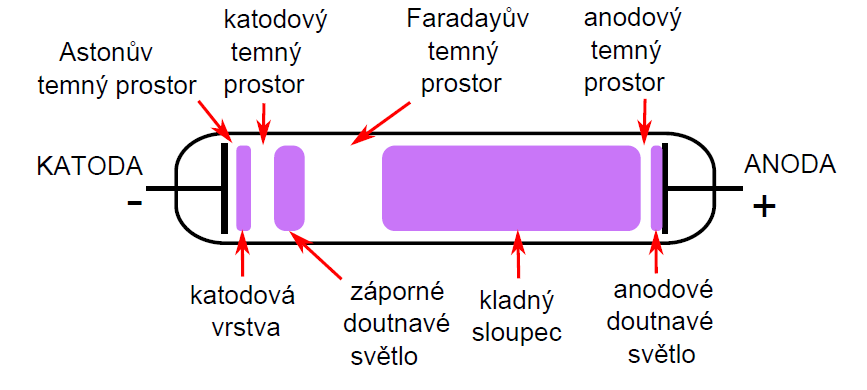
\includegraphics[width=130mm]{glowdischarge.png}
	\caption{Schéma doutnavého výboje.}
	\label{glowdischarge}
\end{figure}

Výboj můžeme charakterizovat voltampérovou (VA) charakteristikou. Ta pro samostatný výboj je vidět na obr. \ref{VA}. Za změnu proudu při konstantním napětí u bodu B je zodpovědný prostorový náboj, kvůli němuž dojde ke změně původního elektrického pole. To nové může podporovat ionizaci ve výboji, což způsobí další růst proudu, přičemž napětí na elektrodách může klesat a vznikne tak část charakteristiky mezi body B a C. Specifická oblast charakteristiky je mezi body C a D, zvyšování proudu zde nelze vysvětlit nárůstem driftové rychlosti nabitých částic. Musí se zde měnit celkový počet částic procházejících průřezem výbojky. Celkový počet částic $N$ lze napsat jako

\begin{equation}
	N = \int n \text{d}S
	\label{10}
\end{equation}

kde $n$ je koncentrace nabitých částic ve výboji a $S$ je plocha, kterou zabírá záporné světlo na katodě. V katodové oblasti normálního doutnavého výboje vzrůstá $N$ v důsledku růstu $S$, v kladném sloupci však vzrůstá koncentrace $n$. Napětí ve výbojce se skládá z napětí v katodové oblasti a ze spádu napětí na katodovém sloupci, který se s rostoucím proudem zvyšuje. Pokud vzroste proud tak, že celá katoda je pokryta záporným světlem, přechází doutnavý výboj do takzvaného anomálního stavu. Napětí v katodové oblasti roste rychleji než napětí v kladném sloupci klesá, výsledkem je oblast charakteristiky od bodu D k E. Oblast E-F odpovídá přechodu na obloukový výboj.

Katodový spád potenciálu $U_k$ je označení pro napětí mezi ostrou hranicí záporného světla a katodou. Je funkcí materiálu elektrod a plynu ve výbojce. 

\begin{figure}[h]
	\centering
	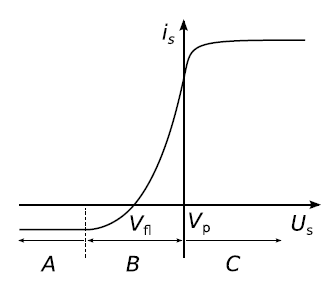
\includegraphics[width=130mm]{VA.png}
	\caption{Voltampérová charakteristika samostatného výboje.}
	\label{VA}
\end{figure}




\section{Měření a výsledky}
\subsection{Paschenův zákon}
Pro měření použijeme výbojku s pohyblivými elektrodami. Tlak měříme Piraniho manometrem, zápalné napětí určujeme voltmetrem s vysokým vstupním odporem. Plyn ve výbojce je vzduch, kalibrační faktor k Piraniho manometru je tedy 1. První měření provedeme s konstantním tlakem $p = 100\,\si{\pascal}$ , přičemž budeme měnit vzdálenost elektrod od 2\,\si{\milli\meter} do 50\,\si{\milli\meter}. Na výbojce zvyšujeme napětí a odečítáme hodnotu napětí v okamžiku zapálení výboje. Mezi každým měřením vyčkáváme alespoň jednu minutu na rekombinaci náboje ve výbojce. Výsledný graf závislosti $U_z = f(pd)$ je na obr. \ref{tlakfixed}. Body jsou proloženy funkcí podle rovnice (\ref{9}) a dostáváme $B = 440,68 \pm 94,46$ a $C' = 1,68 \pm 0,03$. Výsledky měření se od ideální závislosti popsané rovnicí (\ref{9}) docela odchylují. Tato ochylka může být způsobena jak nepřesností odečítání zápalného napětí, tak nedostatečnou rekombinací nábojů mezi jednotlivými měřeními. 

Druhé měření je za konstantní vzdálenosti elektrod $d = 20\,\si{\milli\meter}$, měníme tlak od 25\,\si{\pascal} do 300\,\si{\pascal}. Opět zapisujeme hodnotu napětí v okamžiku zapálení výboje. Graf závislosti $U_z = f(pd)$ je na obr. \ref{dfixed}. Body jsou proloženy funkcí podle rovnice (\ref{9}) a dostáváme $B = 286,26 \pm 27,22$ a $C' = 0,79 \pm 0,01$. Toto měření se oproti předchozímu více blíží ideální závislosti popsané rovnicí (\ref{9}), z grafu vidíme až na malou odchylku typickou závislost napětí na součinu tlaku a vzdálenosti elektrod.

% UZ ZJISTIT A OKOMENTOVAT, Z MINIMA FCE NEBO MĚŘENÍ?

\begin{figure}[h]
	\centering
	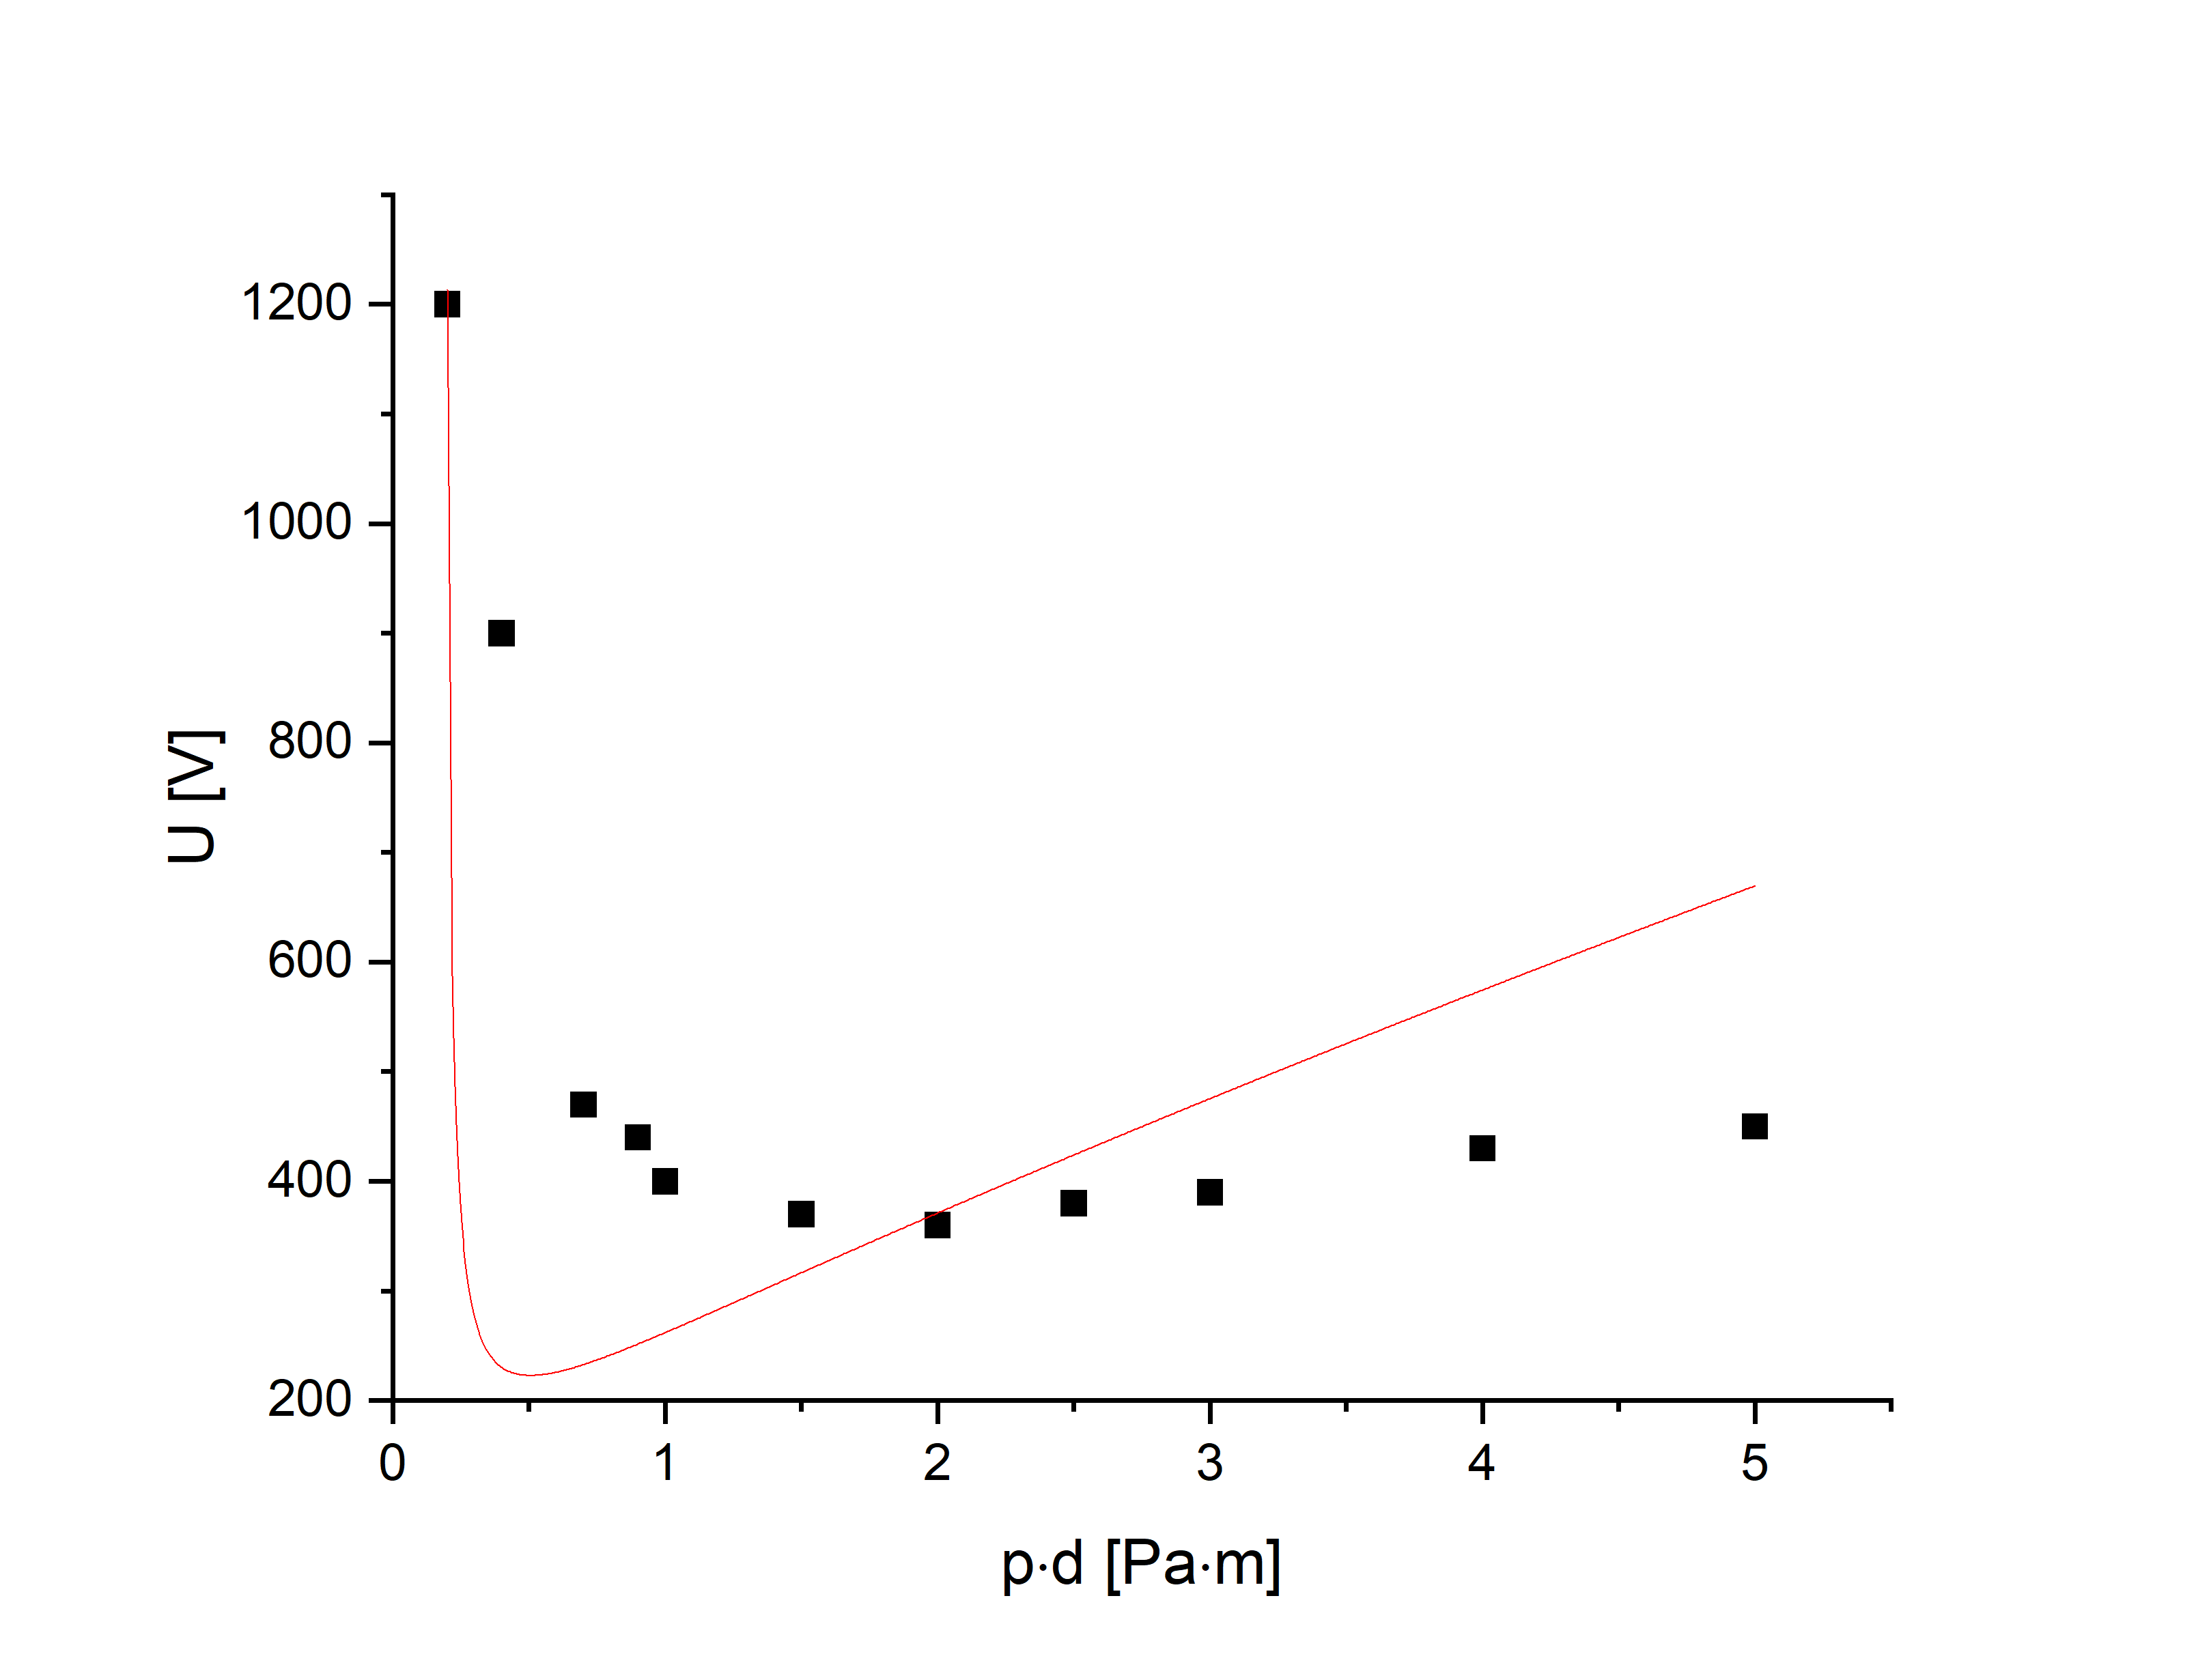
\includegraphics[width=130mm]{tlakfixed.png}
	\caption{Naměřená Paschenova křivka při konstantním tlaku.}
	\label{tlakfixed}
\end{figure}


\begin{figure}[h]
	\centering
	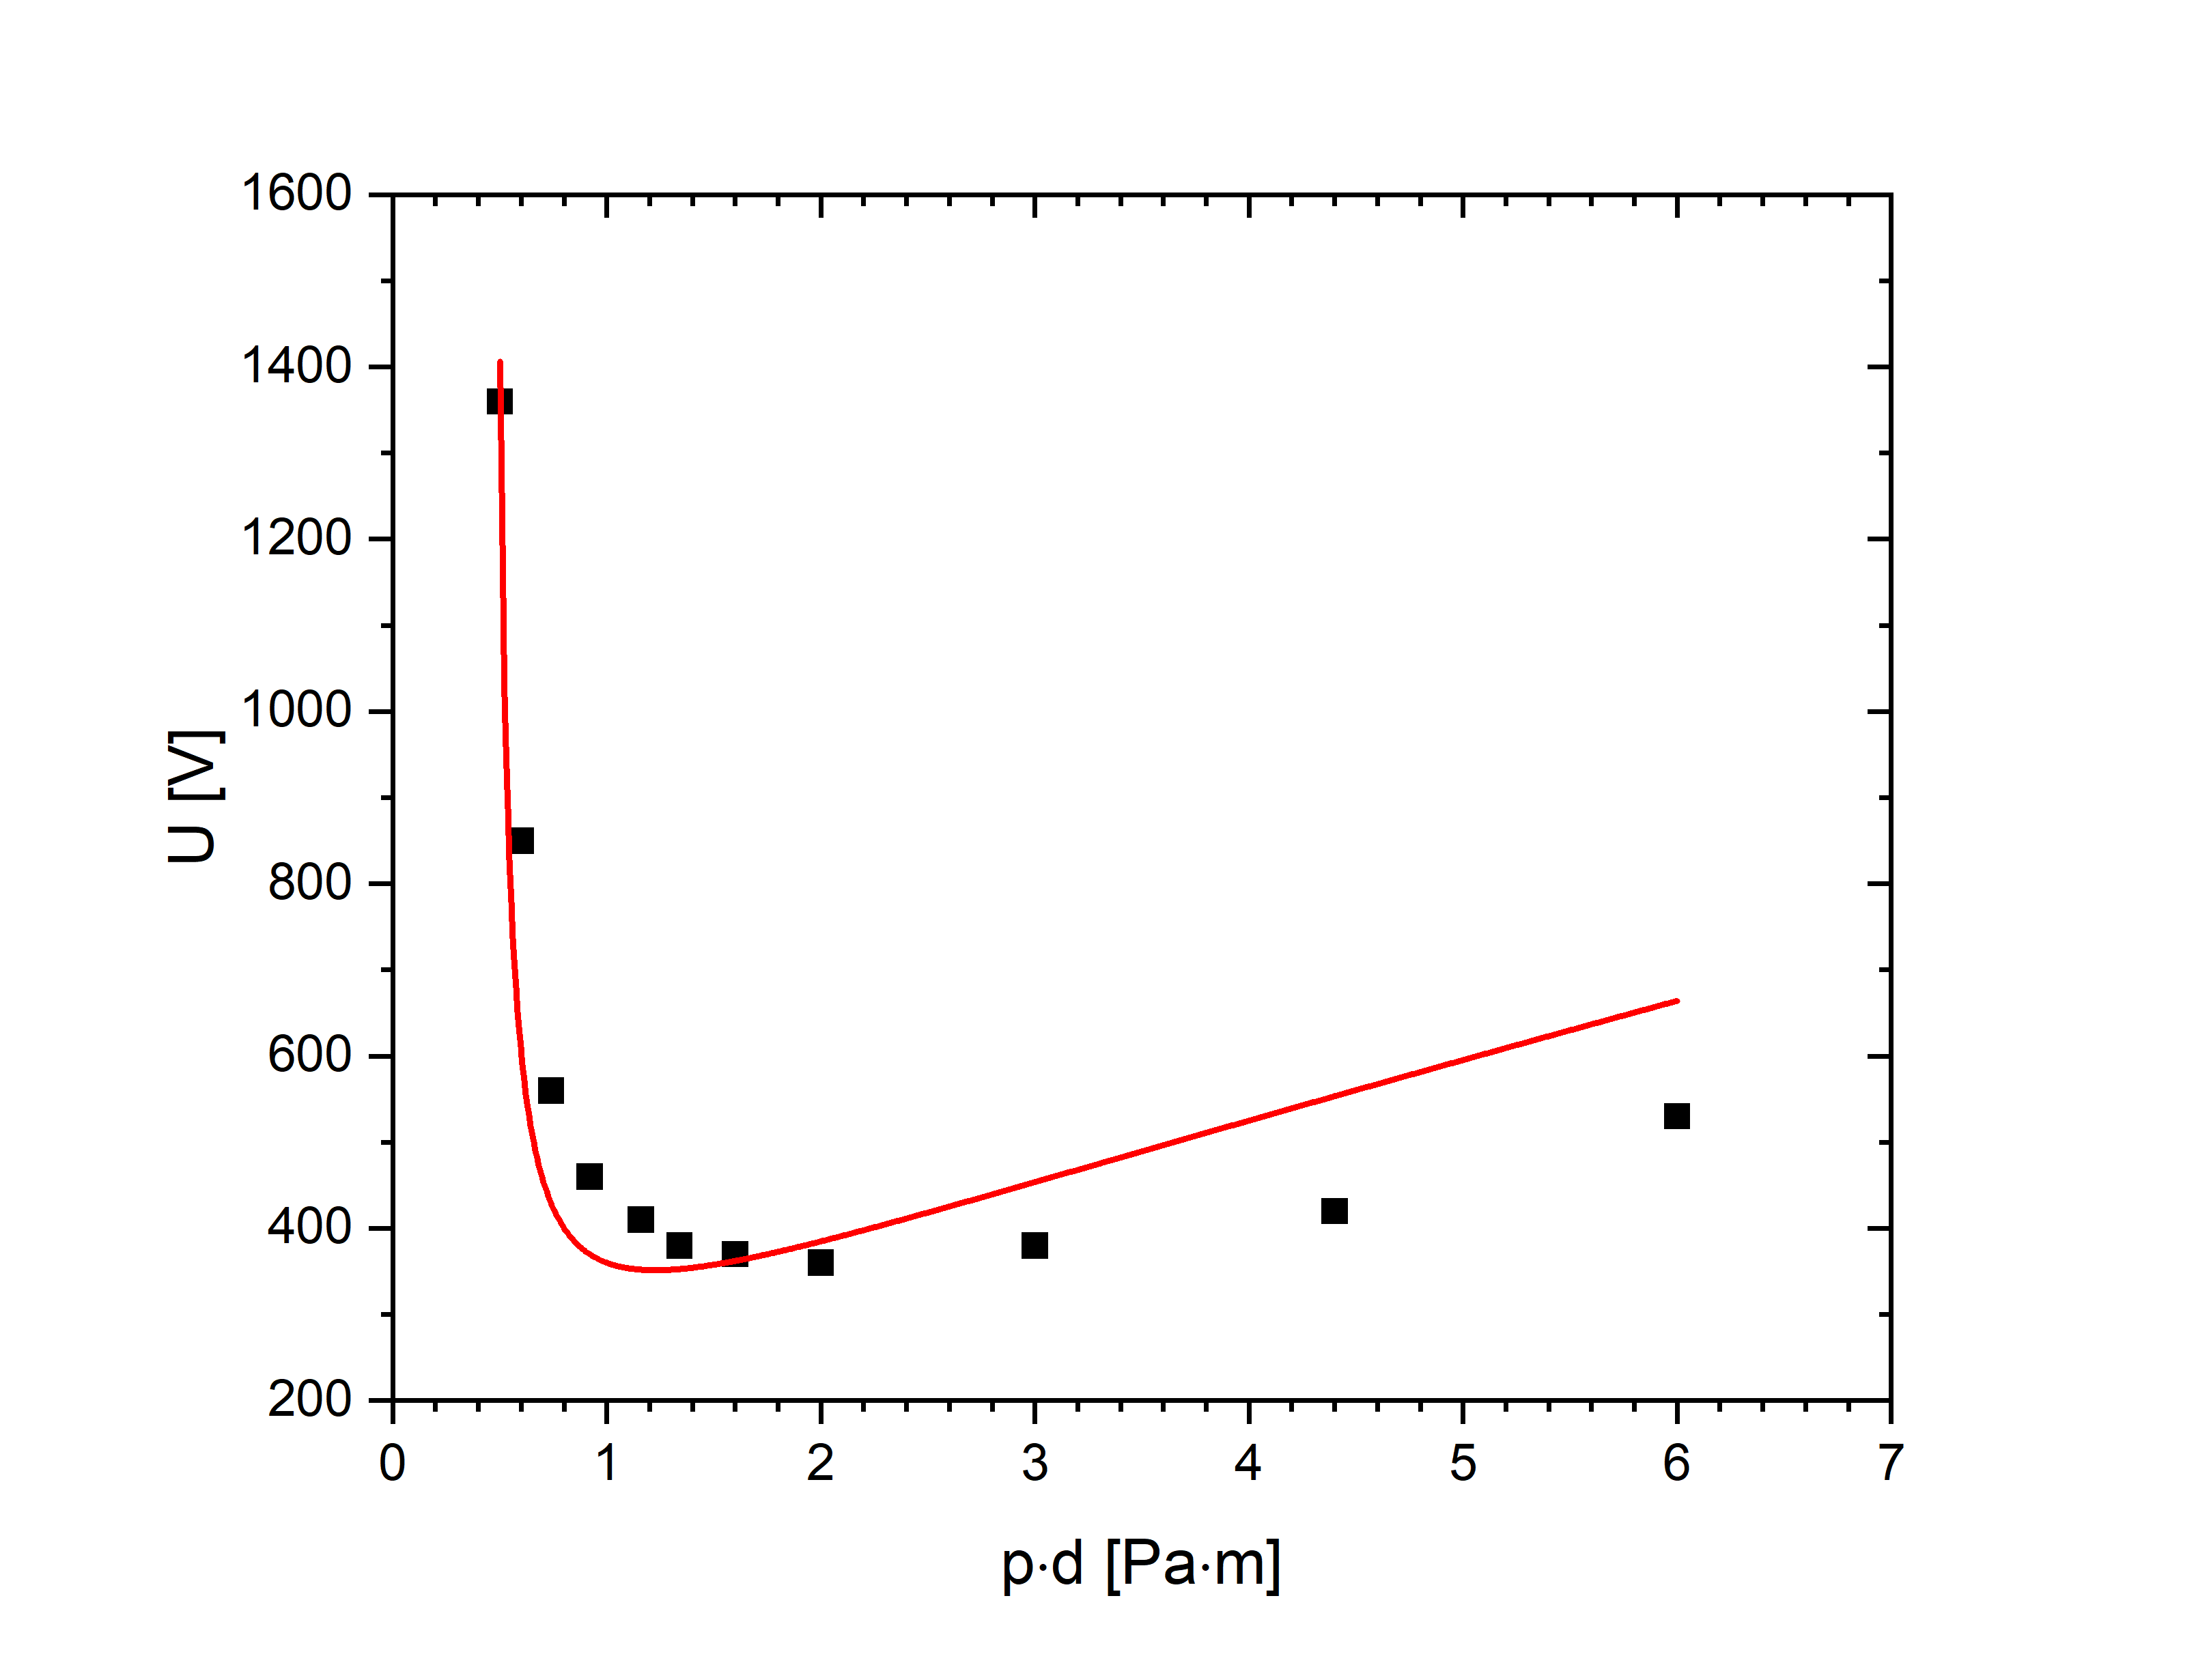
\includegraphics[width=130mm]{dfixed.png}
	\caption{Naměřená Paschenova křivka při konstantní vzdálenosti elektrod.}
	\label{dfixed}
\end{figure}

\subsection{Katodový spád potenciálu v doutnavém výboji}
Stanovení katodového spádu potenciálu provedeme metodou ztíženého výboje. Výbojový proud udržujeme konstantní, měníme vzdálenost elektrod a zapisujeme napětí. Když se anoda dostane do oblasti záporného světla, zmizí anodové světlo. Dalším zmenšováním vzdáleností elektrod začne napětí prudce růst. Napětí vzroste, protože je ztížená ionizace v důsledku zmizení anodového světla, které tedy hraje důležitou roli v mechanizmu vytváření katodového spádu. Měření provedeme pro dvě konstantní hodnoty tlaku a proudu, zaznamenáváme změnu napětí se změnou vzdálenosti elektrod. V grafu na obr. \ref{KatodovySpad} jsou vidět naměřené závislosti. Pro $I = 1\,\si{\milli\ampere}$ a $p = 33\,\si{\pascal}$ je katodový spád $U_k = 701\,\si{\volt}$. Pro $I = 1,8\,\si{\milli\ampere}$ a $p = 100\,\si{\pascal}$ je katodový spád nižší,  $U_k = 514\,\si{\volt}$.  

%komentář proč se katodový spád liší
%komentář vizuál výboje
\begin{figure}[h]
	\centering
	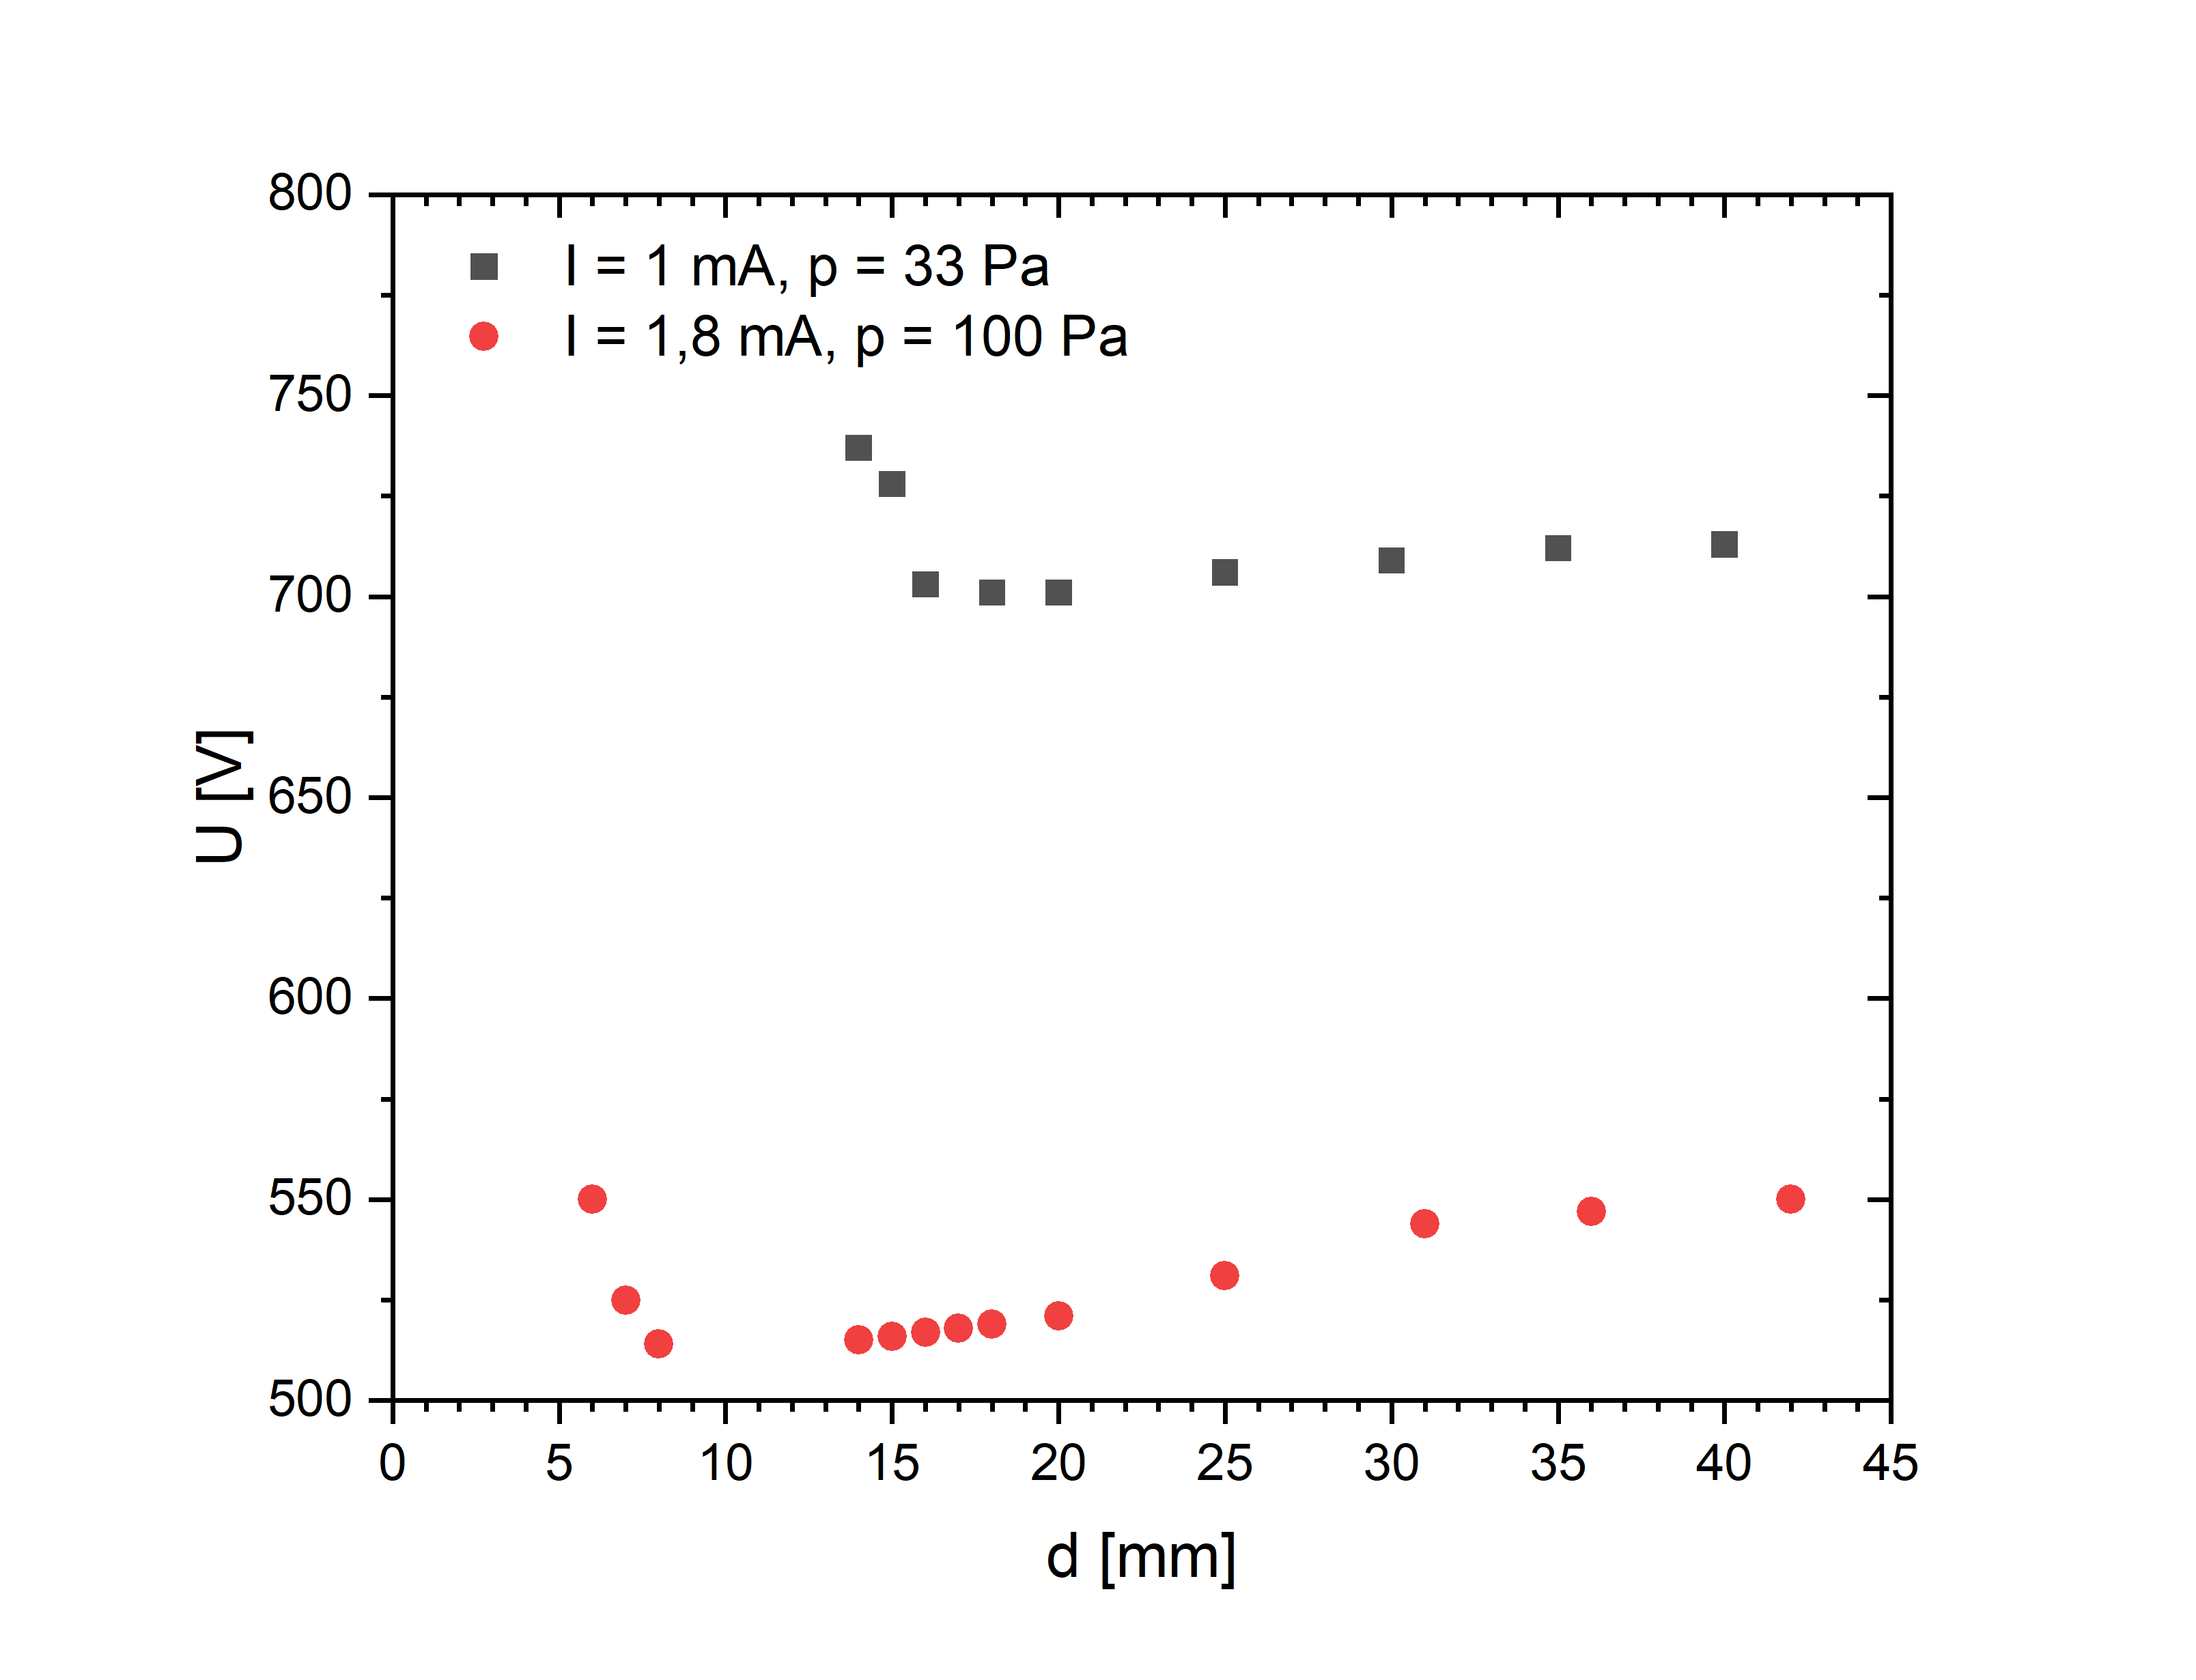
\includegraphics[width=130mm]{KatodovySpad.png}
	\caption{Závislosti napětí na vzdálenosti elektrod, kde minimum napětí odpovídá katodovému spádu.}
	\label{KatodovySpad}
\end{figure}

\section{Závěr}

\end{document}
